\documentclass{article}
\usepackage{../assignment_preamble}

\title{Digit classification using the nearest centroid and PCA algorithms}
\author{Ravi Kini}
\date{December 12, 2025}

\begin{document}

\maketitle

\section{Introduction}
Performing optical character recognition, or OCR, requires that a computer be able to classify handwritten glyphs despite variation in how a glyph is written. Several algorithms for performing this classification exist; this paper focuses on the comparative performance of the nearest centroid and principal component analysis (PCA) algorithms in classifying handwritten digits.

Both the training and testing data sets are sourced from the MNIST database. Images are represented as $28 \times 28$ grayscale pixels grids and stored as $1 \times 784$ vectors. Both data sets are separated by the digit represented. Figure \ref{fig:digit_variation} shows a sample of the images from the training data. Approximately $60,000$ images are present in the training set and $10,000$ in the testing set, with each digit represented roughly equally.

\begin{figure}[!htbp]\label{fig:digit_variation}
    \centering
    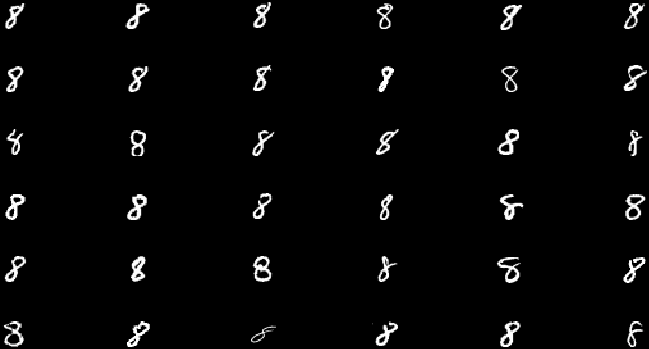
\includegraphics[width=0.5\textwidth]{../../img/ecs130/final/digit_variation.png}
    \caption{Sample images from the training data labeled as representing the digit ``8''.}
\end{figure}

\section{Background}
Let the training set be $X = \{\vec{x}_1, \ldots, \vec{x}_n\}$, with associated digit labels $y_1, \ldots, y_n \in \{0, \ldots, 9\}$. Let $D_j = \{\vec{x}_i \in X : y_i = j\}$, the set of samples from the training set labelled $j$, and let $M_j$ be the matrix with the elements of $D_j$ as its columns.
\subsection{The nearest centroid algorithm}
For the nearest centroid algorithm, we first compute the centroids for each $D_j$:
\begin{align*}
    \vec{\mu}_j = \frac{1}{|D_j|}\sum_{\vec{x} \in D_j} \vec{x}
\end{align*}
\begin{lstlisting}[style=Matlab-editor]
for j = 1:10
    T(j,:) = mean(train{j});
end
\end{lstlisting}
Figure \ref{fig:digit:centroid} shows the pixel grid representation of the centroid fo each digit. To capture how close $\vec{x}$ from the testing set is to each of the centroids, we take the Euclidean norm of the difference between $\vec{x}$ and each $\vec{\mu}_j$. To classify $\vec{x}$, we select the digit associated with the centroid that has the smallest norm.

\begin{align*}
    \hat{y} = \underset{j \in \{0, \ldots, 9\}}{\mathrm{arg~min}} ||\vec{x} - \vec{\mu}_j||_2 
\end{align*}

\begin{lstlisting}[style=Matlab-editor]
for j=1:10
    dist(j) = norm(x - mu(j,:));
end
[~, I] = min(dist);
y_hat = I - 1;
\end{lstlisting}

\begin{figure}[!htbp]\label{fig:digit_centroid}
    \centering
    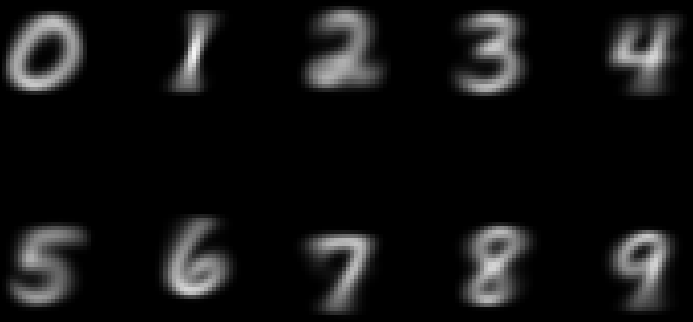
\includegraphics[width=0.5\textwidth]{../../img/ecs130/final/digit_centroid.png}
    \caption{Visual representations of the centroids of each of the digits.}
\end{figure}

\subsection{The PCA algorithm}
For the PCA algorithm, we first compute the singular value decomposition (SVD) of each $M_j$:
\begin{align*}
    M_j & = U_j\Sigma_jV_j^T
\end{align*}
and use the left singular vectors associated with the $m$ largest singular values of $M_j$ as a basis for classification, $U_j^{(m)}$.
\begin{lstlisting}[style=Matlab-editor]
U = zeros(28*28, m, 10);
for j=1:10
    [U_,~,~] = svds(double(train{j})', m);
    U(:,:,j)=U_;
end
\end{lstlisting}
To capture how well $\vec{x}$ from the testing set is represented by $U_j^{(m)}$, we solve the least squares problem:
\begin{align*}
    \underset{\vec{z}}{\min} \left|\left|\vec{x} - U_j^{(m)}\vec{z}\right|\right|_2
\end{align*}
The solution is given by:
\begin{align*}
    \underset{\vec{z}}{\min} \left|\left|\vec{x} - U_j^{(m)}\vec{z}\right|\right|_2 & = \left|\left|\vec{x} - U_j^{(m)}\left(U_j^{(m)}\right)^T\vec{x}\right|\right|_2
\end{align*}
To classify $\vec{x}$, we select the digit associated with the solution that has the smallest norm.

\begin{align*}
    \hat{y} = \underset{j \in \{0, \ldots, 9\}}{\mathrm{arg~min}} \left|\left|\vec{x} - U_j^{(m)}\left(U_j^{(m)}\right)^T\vec{x}\right|\right|_2
\end{align*}

\begin{lstlisting}[style=Matlab-editor]
for j=1:10
    Uj = Us(:,:,j);
    dist(j) = norm(z - Uj*(Uj'*z));
end
[M, I] = min(dist);
y_hat(i) = I - 1;
\end{lstlisting}

\section{Results}
The nearest centroid classifier runs in approximately $0.2$ seconds. Table \ref{tab:confusion_centroid} shows the confusion matrix, with zeros omitted.

\begin{table}[!htbp]
    \centering
    \resizebox{\textwidth}{!}{
    \begin{tabular}{|c|cccccccccc|}
        \hline
        & 0 & 1 & 2 & 3 & 4 & 5 & 6 & 7 & 8 & 9 \\
        \hline
        0 & 0.896 &  & 0.007 & 0.002 & 0.002 & 0.059 & 0.026 & 0.001 & 0.007 & \\
        1 &  & 0.962 & 0.009 & 0.003 &  & 0.006 & 0.003 &  & 0.018 & \\
        2 & 0.018 & 0.069 & 0.757 & 0.032 & 0.03 & 0.003 & 0.022 & 0.017 & 0.048 & 0.003 \\
        3 & 0.004 & 0.024 & 0.025 & 0.806 & 0.001 & 0.049 & 0.008 & 0.015 & 0.057 & 0.012 \\
        4 & 0.001 & 0.022 & 0.002 &  & 0.826 & 0.003 & 0.016 & 0.001 & 0.01 & 0.118 \\
        5 & 0.012 & 0.071 & 0.002 & 0.132 & 0.024 & 0.686 & 0.03 & 0.011 & 0.015 & 0.017 \\
        6 & 0.019 & 0.028 & 0.023 &  & 0.032 & 0.033 & 0.863 &  & 0.001 & \\
        7 & 0.002 & 0.057 & 0.021 & 0.001 & 0.019 & 0.002 &  & 0.833 & 0.013 & 0.052 \\
        8 & 0.014 & 0.04 & 0.011 & 0.085 & 0.012 & 0.037 & 0.013 & 0.01 & 0.737 & 0.039 \\
        9 & 0.015 & 0.022 & 0.007 & 0.01 & 0.082 & 0.012 & 0.001 & 0.027 & 0.018 & 0.807 \\
        \hline
    \end{tabular}}
    \caption{The confusion matrix for the nearest centroid classification algorithm.}
    \label{tab:confusion_centroid}
\end{table}

The digit ``5'' is by far the most often misclassified, being consistently confused with ``3''. On the other hand, ``1'' is the most consistently correct classified digit.

The PCA classifier runs in approximately $0.5$ seconds for $m = 1$, $0.9$ seconds for $m = 5$, $1.4$ seconds for $m = 10$, and $1.8$ seconds for $m = 20$, exhibiting a roughly linear dependence on $m$. For $m = 1$, the PCA algorithm performs on par with the nearest centroid classifier. Table \ref{tab:confusion_pca} shows the confusion matrix, with zeros omitted.

\begin{table}[!htbp]
    \centering
    \resizebox{\textwidth}{!}{
    \begin{tabular}{|c|cccccccccc|}
        \hline
        & 0 & 1 & 2 & 3 & 4 & 5 & 6 & 7 & 8 & 9 \\
        \hline
        0 & 0.92 &  & 0.005 & 0.004 &  & 0.032 & 0.026 & 0.001 & 0.012 &  \\
        1 &  & 0.937 & 0.007 & 0.004 &  & 0.003 & 0.004 &  & 0.045 &  \\
        2 & 0.025 & 0.043 & 0.747 & 0.052 & 0.025 &  & 0.032 & 0.015 & 0.056 & 0.005\\
        3 & 0.006 & 0.005 & 0.026 & 0.834 &  & 0.036 & 0.009 & 0.013 & 0.055 & 0.017 \\
        4 & 0.004 & 0.011 & 0.003 &  & 0.797 & 0.001 & 0.024 & 0.001 & 0.021 & 0.136 \\
        5 & 0.03 & 0.031 & 0.015 & 0.118 & 0.028 & 0.649 & 0.035 & 0.015 & 0.053 & 0.027 \\
        6 & 0.03 & 0.016 & 0.019 & 0.001 & 0.018 & 0.022 & 0.884 &  & 0.01 &  \\
        7 & 0.008 & 0.049 & 0.024 &  & 0.016 &  & 0.001 & 0.819 & 0.023 & 0.06 \\
        8 & 0.006 & 0.022 & 0.011 & 0.093 & 0.011 & 0.031 & 0.017 & 0.008 & 0.764 & 0.036 \\
        9 & 0.018 & 0.017 & 0.007 & 0.012 & 0.078 & 0.01 & 0.002 & 0.028 & 0.026 & 0.803 \\
        \hline
    \end{tabular}}
    \caption{The confusion matrix for the PCA algorithm, with $m =1$.}
    \label{tab:confusion_pca}
\end{table}

Like the nearest centroid classifier, ``1'' is the most consistently correctly classified, and ``5'' the least, with it often being confused with $3$. For higher values of $m$, the PCA classifier performs much more consistently, with at least 88\% accuracy for all digits. The accuracies are summarized in Table \ref{tab:accuracy}

\begin{table}[!htbp]
    \centering
    \resizebox{\textwidth}{!}{
    \begin{tabular}{|c|cccccccccc|}
        \hline
        (\%) & 0 & 1 & 2 & 3 & 4 & 5 & 6 & 7 & 8 & 9 \\
        \hline
        Nearest centroid & 89.6 & 96.2 & 75.7 & 80.6 & 82.6 & 68.6 & 86.3 & 83.3 & 73.7 & 80.7 \\
        \hline
        PCA, $m = 1$ & 92.0 & 93.7 & 74.7 & 83.4 & 79.7 & 64.9 & 88.4 & 81.9 & 76.4 & 80.3 \\
        PCA, $m = 5$ & 97.9 & 99.2 & 90.2 & 93.8 & 89.8 & 90.1 & 96.2 & 89.3 & 90.0 & 88.9 \\
        PCA, $m = 10$ & 98.8 & 99.5 & 92.7 & 94.3 & 95.6 & 91.9 & 96.6 & 93.4 & 91.8 & 93.3 \\
        PCA, $m = 20$ & 98.8 & 99.4 & 93.5 & 94.2 & 96.8 & 93.9 & 97.5 & 94.6 & 94.4 & 93.9 \\
        \hline
    \end{tabular}}
    \caption{Accuracy rates for the nearest centroid and PCA classifiers.}
    \label{tab:accuracy}
\end{table}

Even for high values of $m$, ``5'' remains among the least consistently correctly classified, and ``1'' among the most by the PCA classifier. Notably, increasing $m$ also has less of an effect for higher values of $m$, indicating that including more left singular vectors in the basis has diminishing returns.

\section{Conclusion}
Overall, the PCA classifier performs much better than the nearest centroid classifier for sufficiently large $m$, although it is also more computationally expensive. The accuracy still remains, however, below human level\footnote{\textit{Advances in Neural Information Processing Systems} (Simard, LeCun, and Denker 1992)}; reaching and surpassing this threshold requires the use of more sophisticated techniques, like support vector machines.

\appendix

\section{Code}
\begin{lstlisting}[style=Matlab-editor,title=main.m]
clear;
load mnistdata;

for j=1:10
    train{j} = eval(['train' num2str(j-1)]);
    test{j} = eval(['test' num2str(j-1)]);
end

figure(1)
m = 6; % display the selected train/test digits in an m x m array
for i = 1:m*m
    digit = train8(i,:);
    %digit = test8(i,:);
    digitImage = reshape(digit,28,28);
    subplot(m,m,i);
    image(rot90(flipud(digitImage),-1));
    colormap(gray(256));
    axis square tight off;
end

for j = 1:10
    mu(j,:) = mean(train{j});
end

for i = 1:10
    digitImage_mean(:,:,i) = reshape(mu(i,:),28,28);
end
figure(2)
for i = 1:10
    subplot(2,5,i)
    image(rot90(flipud(digitImage_mean(:,:,i)),-1));
    colormap(gray(256));
    axis square tight off;
end

confusion_centroid = zeros(10, 10);
for i=1:10
    centroid_classify{i} = mycentroid(test{i}, mu);
    success_rate_centroid(i) = sum(centroid_classify{i} == (i - 1)) / numel(centroid_classify{i}) * 100;
    for j=1:10
        confusion_centroid(i,j) = round(sum(centroid_classify{i} == (j - 1)) / numel(centroid_classify{i}), 3);
    end
end

fprintf('centroid classification\n');
pretty_print(success_rate_centroid);

for m = [1, 5, 10, 20]
    if m == 1
        confusion_pca = zeros(10, 10);
    end
    U = zeros(28*28, m, 10);
    for j=1:10
        [U_,~,~] = svds(double(train{j})', m);
        U(:,:,j)=U_;
    end
    
    for i=1:10
        pca_classify{i} = mypca(test{i}, U);
        success_rate_pca(i) = sum(pca_classify{i} == (i - 1)) / numel(pca_classify{i}) * 100;
        for j=1:10
            confusion_pca(i,j) = round(sum(pca_classify{i} == (j - 1)) / numel(pca_classify{i}), 3);
        end
    end
    fprintf('principal component analysis classification (m = %i)\n', m);
    pretty_print(success_rate_pca);
end
\end{lstlisting}

\begin{lstlisting}[style=Matlab-editor,title=mycentroid.m]
function [y_hat] = mycentroid(x, mu)
    n = size(x,1);
    for i=1:n
        x_ = double(x(i,:));
        dist = zeros(10,1);
        for j=1:10
            dist(j) = norm(x_ - mu(j,:));
        end
        [~, I] = min(dist);
        y_hat(i) = I - 1;
    end
end
\end{lstlisting}

\begin{lstlisting}[style=Matlab-editor,title=mypca.m]
function [y_hat] = mypca(x, Us)
    n = size(x,1);
    for i=1:n
        z = double(x(i,:))';
        dist = zeros(10,1);
        for j=1:10
            Uj = Us(:,:,j);
            dist(j) = norm(z - Uj*(Uj'*z));
        end
        [M, I] = min(dist);
        y_hat(i) = I - 1;
    end
end
\end{lstlisting}

\begin{lstlisting}[style=Matlab-editor,title=prettyprint.m]
function pretty_print(success_rate)
    fprintf('-------------');
    for i = 0:9
        fprintf('--------');
    end
    fprintf('\ndigit        |');
    for i = 0:9
        fprintf(' %i     |', i);
    end
    fprintf('\nsuccess rate |');
    for i = 1:10
        fprintf(' %.1f%% |', success_rate(i));
    end
    fprintf('\n-------------');
    for i = 0:9
        fprintf('--------');
    end;
    fprintf('\n');
end
\end{lstlisting}
\end{document}